\documentclass{article}
\usepackage[utf8]{inputenc}
\usepackage{mathtools}
\usepackage{amssymb}
\usepackage{graphicx}
\usepackage{listings}
\usepackage{float}
\usepackage{gensymb}
\usepackage{amsthm}
\usepackage{longtable}
\usepackage{adjustbox}
\usepackage{physics}
\usepackage{dsfont}
\usepackage{cancel}

\theoremstyle{definition}
\newtheorem{definition}{Definition}
\newtheorem{example}{Example}
\newtheorem{theorem}{Theorem}
\newtheorem{claim}{Claim}

\title{Quantum Information Theory}
\author{quinten tupker}
\date{January 22 2021 - \today}

\begin{document}

\maketitle

\section*{Introduction}

These notes are based on the course lectured by Professor Matthew Wingate in
Lent 2020. 
This was lectured online due to measures taken to counter the spread of Covid-19
in the UK. These are not necessarily an accurate representation of what was
lectures, and represent solely my personal notes on the content of the course,
combinged with probably, very very many personal notes and digressions... Of
course, any corrections/comments would be appreciated.

[the lecturer outlines the course] This course is an extension of the Michaelmas
Quantum Field Theory course that introduces renormalisation and the path
integral formulation of quantum field theory.

\section*{The Path Integral in Quantum Mechanics}

We start by reformulating the Schr\"{o}dinger equation as an integral equation,
which turns out to be a path integral. Anyways, starting with Schr\"{o}dinger's
equation for a Hamiltonian $H(x, p), [x, p] = i\hbar$ with

\begin{equation}
  H = \frac{p^2}{2m} + V(x)
\end{equation}

we have

\begin{equation}
  i\hbar \partial_t \ket{\psi(t)} = H \ket{\psi(t)} \implies \ket{\psi(t)} = e^{-i H t / \hbar}
  \ket{\psi(0)}
\end{equation}

where in the Schr\"{o}dinger picture the states evolve, but the operators remain
constant, and the wavefunction $\Psi(x, t) = \bra{x} \ket{\psi(t)}$. As such we
can rewrite our equation as

\begin{equation}
  \bra{x} H \ket{\psi(x)} = \left( \frac{-\hbar^2}{2m} \partial_x^2 + V(x) \right) \bra{x} \ket{\psi(t)}
\end{equation}

so we can write

\begin{align*}
  \Psi(x, t) &= \bra{x} \ket{\psi(t)} \\
             &= \bra{x} e^{-i H t / \hbar} \ket{\psi(0)} \\
             &= \int_{-\infty}^\infty dx_0 \bra{x} e^{-i H t / \hbar} \ket{x_0} \bra{x_0} \ket{\psi(0)} \\
             &= \int_{-\infty}^\infty dx_0 K(x, x_0, t) \Psi(x_0, 0)
\end{align*}

for \textbf{kernel} $K(x, x_0, t) = \bra{x} e^{-i H t / \hbar} \ket{x_0}$. Now,
if it is hard to calculate $K$ for large $t$, it can be beneficial to split this
into many intervals for many values of $t$, such as $0 = t_0 < t_1 < \dots < t_n
< t_{n + 1} = T$ leaving

\begin{equation}
  K(x, x_0, T) = \int_{-\infty}^\infty \prod_{r = 1}^n dx_r \bra{x_{r + 1}} e^{- iH(t_{r + 1} - t_r) / \hbar} \ket{x_r} \bra{x_1} e^{-iH (t_1 - t_0) / \hbar} \ket{0}
\end{equation}

which is in a sense an integral over all possible sequences of values of $x$. 

In free field theory ($V = 0$) this can be explicitly evaluated using a Gaussian
integral by rewriting things in the momentum basis as (use $\bra{x} \ket{p} =
e^{i px / \hbar}$)

\begin{align*}
  K_0(x, x', t) &= \bra{x} e^{\frac{-i p^2 t}{2m \hbar}} \int \frac{dp}{2\pi \hbar} \ket{p} \bra{p} \ket{x'} \\
                &= \int_{-\infty}^\infty \frac{dp}{2 \pi \hbar} e^{\frac{-ip^2 t}{2m \hbar}} e^{ip (x - x') / \hbar}\\
                &= e^{\frac{ip(x - x')^2}{2\hbar t}} \sqrt{\frac{m}{2\pi i \hbar t}}
\end{align*}

where we note that the limit as $t \to 0$ is $\delta(x - x')$ which indeed
matches $\bra{x} \ket{x'} = \delta(x - x')$ as expected.

Now in an interacting theory, we struggle with the Baker-Campbell-Hausdorff fact
that $e^A e^B \neq e^{A + B}$ so using Suzuki-Trotter we separate into steps
size $t_{r + 1} - t_r = \delta t << T$ meaning that

\begin{equation}
  e^{-iH \delta t / \hbar} \approx e^{\frac{-ip^2 \delta t}{2m \hbar}} e^{\frac{-i V(x) \delta}{\hbar}} (1 + O(\delta t^2))
\end{equation}

so for $T = n \delta t$ we find that

\begin{equation}
  K(x, x_0, T) = \int \prod_{r = 1}^n dx_r \left( \frac{m}{2\pi i \hbar \delta t} \right)^{\frac{n + 1}{2}}
  e^{i \sum_{r = 0}^n \left( \frac{m}{2 \hbar} \left( \frac{x_{r + 1} - x_r}{\delta t} \right)^2
      - V(x_r) / \hbar \right) \delta t}
\end{equation}

which in the limit $n \to \infty, \delta t \to 0$ while keeping $T$ constant
leaves

\begin{equation}
  \frac{1}{\hbar} \int_0^T dt \left( \frac{1}{2}m \dot{x}^2 - V(x) \right) = \int_0^T dt L(x, \dot{x}) = S
\end{equation}

for classical Lagrangian $L$ and action $S$. This is what we refer to as a path
integral or function integral:

\begin{equation}
  K(x, x_0, t) = \int \mathcal{D}x e^{i S / \hbar}
\end{equation}

where $\mathcal{D} x$ is the limit describd above. Of course, many questions
about the existence and uniqueness, etc. of such limits exists, and in fact
often this limit does not exist, but in the cases we are interested it, it works
well enough... [End of lecture 1]

We make the following remarks

\begin{itemize}
\item In the classical limit $\hbar \to 0$ the lowest frequencies
  dominate $K$. This is equivalent to Hamilton's principle (the principle of
  least action), as expected.
\item it is common and helpful to extend analytically to imaginary time $\tau =
  it$ leaving $\bra{x} e^{-H\tau / \hbar} \ket{x_0} = \int \mathcal{D}x e^{-S /
    \hbar}$ which has better convergence properties and is easier to interpret
  than the complex version (Hamilton's principle appears more easily as well). 
\end{itemize}

\section{Integrals and their diagrammatic expansion}

The above considered quantum mechanics, which is in a sense the $0 + 1$
dimension vrsion of QFT (since $x$ is treated as an operator, while $t$ is
treated as a variable). To move to more general QFT, we start, strangely, with 0
dimensional QFT, for $\phi : \{ \cdot \} \to \mathbb{R}$ a field on a single
point. Here,

\begin{equation}
  \mathcal{Z} = \int_\mathbb{R} d\phi e^{-S(\phi) / \hbar}
\end{equation}

where we assume $S$ is an even polynomial in $\phi$ for convergence reasons, and
we are interested in expectation values

\begin{equation}
  \langle f \rangle = \frac{1}{\mathcal{Z}} \int d\phi f(\phi) e^{-S(\phi) / \hbar}
\end{equation}

\subsection{Free Theory}

For $N$ fields $\phi_a, a = 1, \dots, N$, let $S(\phi) = \frac{1}{2} \phi^T m
\phi$ for a symmetric positive definite matrix $m = P\Delta P^T$ for orthogonal
$P$. As such, we can write this essentially Gaussian integral as

\begin{equation}
  \mathcal{Z}_0 = \int d^N \phi e^{-\frac{1}{2 \hbar} \phi^T m \phi} = \sqrt{\frac{(2\pi\hbar)^N}{\det m}}
\end{equation}

From here, we can turn this into a generating function to calculate expectation
values by taking derivatives by turning $S_0(\phi) \mapsto S_0(\phi) - J^T
\phi$, and writing $\mathcal{Z}_0 = \mathcal{Z}_0(J)$ (now a generating
function(al) - functional later on). We then remark

\begin{equation}
  \mathcal{Z}_0(J) = \mathcal{Z}_0(0) e^{-\frac{1}{2\hbar} J^T m^{-1} J}
\end{equation}

Then we can calculate the correlation functions as

\begin{equation}
  \langle \phi_a \phi_b \rangle = \frac{1}{Z_0(0)} \hbar^2 \partial_{J_a} \partial_{J_b} \mathcal{Z}_0(J) |_{J = 0}
  = h(m^{-1})_{ab}
\end{equation}

Conveniently, this can be diagrammatically interpreted as a connecting two
vertices on indices $a, b$ with an undirected edge. We can generalise this to
linear operator $l(\phi) = \sum l_a \phi_a$ as (for $p$ such operators)

\begin{equation}
  \langle l^{(1)}(\phi) \dots l^{(p)}(\phi) \rangle = \hbar^p \prod_{i = 1}^p l^{(i)}(\partial_J) e^{\frac{1}{\hbar} J^T m^1 J}
\end{equation}

If $p$ is odd, this is always 0 by symmetry, but if $p$ is even this corresponds
to a linear combination of products $m_{ab}^{-1} m_{cd}^{-1} \dots$

\begin{example}
  For $p=4, l^{(1)}_a = \delta_{ab}, l^{(2)}_a = \delta_{ac}, l^{(3)}_a =
  \delta_{ad}, l^{(4)}_a = \delta_{af}$ then
  \begin{equation}
    \langle \phi_b \phi_c \phi_d \phi_f \rangle = \hbar^2 (m_{bc}^{-1} m_{df}^{-1} + m_{bd}^{-1} m_{cf}^{-1} +
    m_{bf}^{-1} m_{cd}^{-1})
  \end{equation}
  which also corresponds to the ways in which we can connect four vertices with
  undirected edges
  \begin{figure}[H]
    \centering
    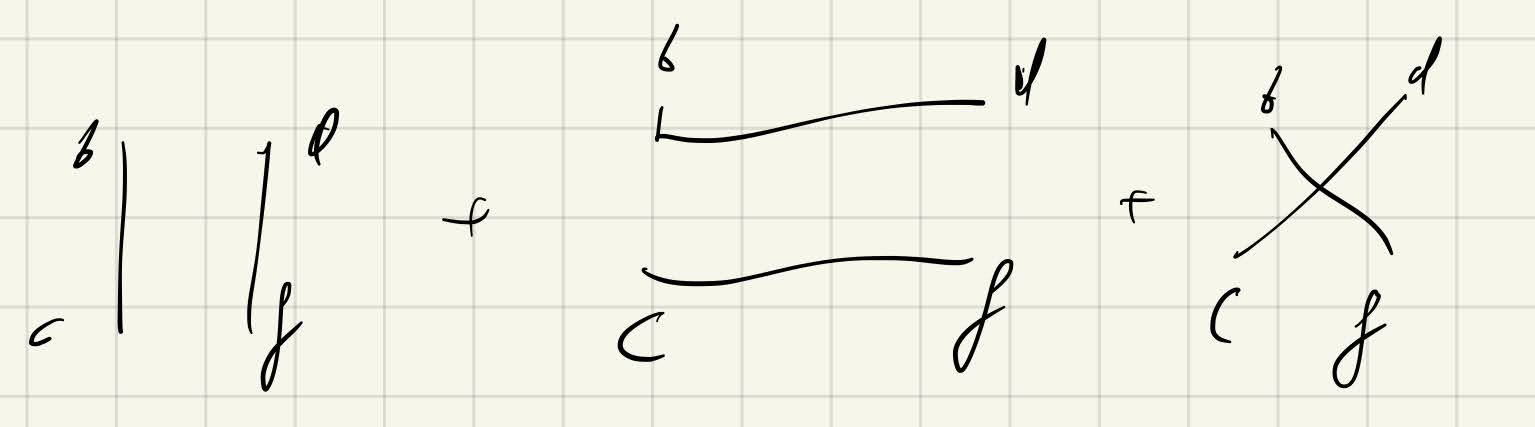
\includegraphics[width=7cm]{res/AQFT/connecting_four_vertices}
    \label{connecting_four_vertices}
  \end{figure}
\end{example}

[End of lecture 2]

\subsection{Interacting Theory}

We start investigating interacting theory by doing a series expansion of

\begin{equation}
  \int_{\mathbb{R}^N} \d^N \phi f(\phi) e^{-S / \hbar}
\end{equation}

in $\hbar$. However, we find that in general, the radius of convergence of these
perturbed series is 0, since if we take $\hbar < 0$ these do not converge. As
such, we get asymptotic behaviour along the lines described by saying that

\begin{definition}
  $I(\hbar)$ is \textbf{asymptotic} to $\sum_{n = 0}^\infty c_n \hbar^n$
  (denoted by $\sim$) if $\lim_{\hbar \to 0^+} \frac{1}{\hbar^N} | I(\hbar) -
  \sum_{n = 0}^N c_n \hbar^n | = 0$ for fixed $N$.
\end{definition}

This is much weaker than convergence since we find that adding new terms may in
fact make things worse. But it does allow us to account for transcendental terms
like $e^{-1 / \hbar^2} ~ 0$ (called \textbf{nonperturbative contributions}).

Now we work out the case where

\begin{equation}
S(\phi) = \frac{1}{2} m^2 \phi^2 + \frac{\lambda}{4!} \phi^4
\end{equation}

and expand about the minimum of $S$ at $\phi=0$ to get

\begin{equation}
\mathcal{Z} = \int d\phi e^{-S / \hbar} = \int d\phi e^{-S / \hbar} 
\sum_v^\infty \frac{1}{v!} \left( \frac{-\lambda}{4! \hbar} \phi^4 \right)^v
\end{equation}

but since we don't converge, we certainly can't swap $\int$ and $\sum$ so here
we first truncate, and then swap. As such, if we write $x = \frac{1}{2\hbar} m^2
\phi^2$,

\begin{equation}
\mathcal{Z} \sim \frac{\sqrt{2\hbar}}{m} \sum_{v = 0}^N \frac{1}{v!} \left( 
\frac{-\hbar \lambda}{4! m^4} \right)^v 2^{2v} \int_0^\infty dx e^x x^{2v
+ 1/2 - 1}
\end{equation}

where the integral is just the gamma function $\Gamma(2v + 1/2) = \frac{(4v)!
  \sqrt{\pi}}{4^{2v} (2v)!}$ so

\begin{equation}
\mathcal{Z} \sim \frac{\sqrt{2\hbar}}{m} \sum_{v = 0}^N \frac{1}{v!} \left( 
\frac{-\hbar \lambda}{4! m^4} \right)^v \frac{1}{(4!) v} \frac{(4v)! \sqrt{\pi}}{2^{2v} (2v)!}
\end{equation}

(the lecture notes seem to omit the $\sqrt{\pi}$). Here the $\frac{1}{(4!) v}$
comes from expanding the interaction term $e^{-S_1 / \hbar}$ and the second
fraction comes from the number of ways to pair $4v$ fields with $v$ copies of
$\phi^4$. Applying stirling's formula, this series grows as $v!$ so this series
is definitely not convergent, but still asymptotic. Now, as before, we want to
insert our $J$ somehow to get a generating function. Here we get

\begin{align*}
\mathcal{Z}(J) &= \int d\phi e^{-\frac{1}{\hbar} (S_0(\phi) + S_1(\phi) - J\phi)} \\
&= e^{-\frac{1}{\hbar} S_1(\hbar \partial_J)} \int d\phi e^{-\frac{1}{\hbar} 
(S_0(\phi) - J\phi)} \\
&\sim e^{-\frac{\lambda}{4! \hbar} (\hbar \partial_J)^4} e^{\frac{1}{2\hbar} J^T m^{-1} J}
\end{align*}

which works out to

\begin{equation}
  \mathcal{Z}(J) \sim \sum_{v=0}^N \frac{1}{v!} \left( \frac{-\lambda}{4! \hbar}
    (\hbar \partial_J)^4 \right)^v \sum_{p = 0} \frac{1}{p!} \left( \frac{1}{2\hbar}
    J^T m^{-1} J \right)^p
\end{equation}

where diagramatically $v$ corresponds to the number of vertices, and $p$ to the
number of propagators.

\begin{figure}[H]
  \centering
  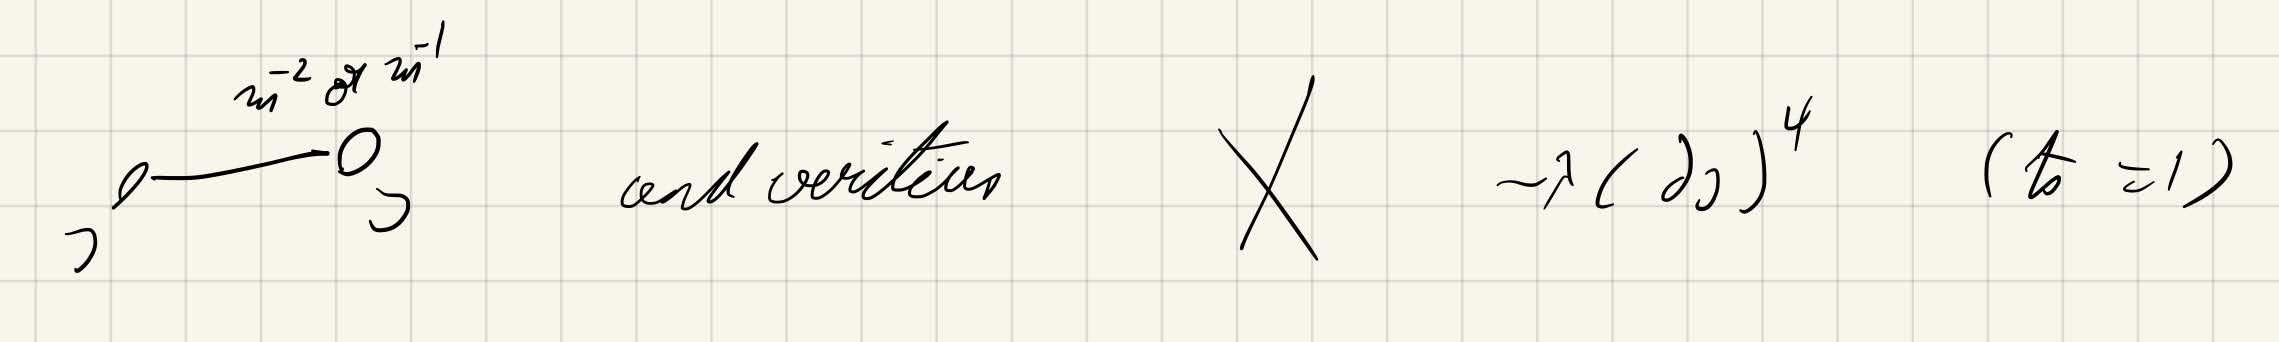
\includegraphics[width=7cm]{res/AQFT/diagram_interpretation}
  \label{diagram_interpretation}
\end{figure}
 
where in order to get a nonzero term we need the number of derivatives ($4v$
vertex line ends - 4 per vertex here) to match the number of sources ($2p$ for
each propagator) to match. However, we can have a predetermined number of
external sources $E = 2p - 4v$. For example, the first two nontrivial terms in
the $Z(0)$ expansion for $E = 0$ are $(v, p) = (1, 2), (2, 4)$ which corresponds
diagrammatically to

\begin{figure}[H]
  \centering
  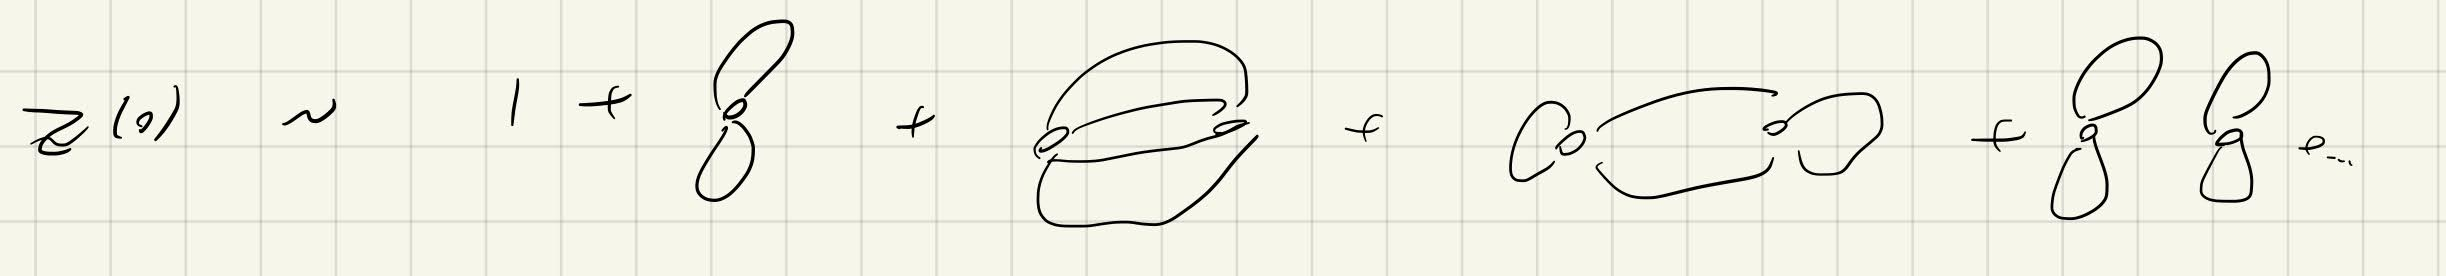
\includegraphics[width=7cm]{res/AQFT/quartic_series_diagram}
  \label{quartic_series_diagram}
\end{figure}

Note that each diagram may have a factor in front of it determined by how often
it repeats itself (affect by the product rule in taking derivatives). [end of
lecture 3]

To work out these prefactors, consider the first non-constant term above, the
figure eight. We can split this into its components: a vertex and two
propagators - it's so-called ``pre-diagram.'' We can work out the prefactor by
considering the number of ways to connect these while still forming a figure
eight, $A = 4!$, and dividing by a denominator given by the coefficients in the
series

\begin{equation}
  F = v! (4!)^v (p!) 2^p = 1 \cdot 4! \cdot 2 \cdot 2^2 = 4! 2^3
\end{equation}

leaving prefactor $A / F = 1 / 8$. Note here that $F$ accounts for

\begin{itemize}
\item $v!$ ways to permute the vertices
\item $4!$ ways to permute the vertex legs
\item $p!$ ways to permute the propagator legs
\item $2^p$ ways to swap propagator direction
\end{itemize}

Now, another interpretation is that $A / F = 1 / S$ where $S$ is the
\textbf{symmetry factor} counting the number of ways of redrawing the unlabelled
graph to leave its overall structure the same (the number of graph
isomorphisms). So, for example, for the figure eight, we get $S = 2 \times 2
\times 2 = 8$ for swapping the direction of loop 1, swapping the direction of
loop 2, and swapping loops 1 and 2. Similarly for the basketball, we get $S = 4!
\cdot 2 = 48$ for $4!$ ways to rearrange the lines and $2$ ways to swap
vertices (what happened to swapping the orientations of the lines?). Working by
brute force, to verify we get $A = 8 \cdot 6 \cdot 4 \cdot 2 \cdot 4! = 3^2
2^{10}$ for the number of ways to connect propagators and the number of their
permutations. Similarly, $F = 2(4!)^24! 2^4 = 3^3 2^{14},$ leaving $A / F = 1 /
48 = 1 / S$. Overall, in this case we get

\begin{equation}
  \mathcal{Z}(0) / \mathcal{Z}_0(0) = 1 - \frac{\hbar \lambda}{8m^4} +
  \frac{\hbar^2 \lambda^2}{m^8} \left( \frac{1}{48} + \frac{1}{16} +
    \frac{1}{128} \right) + O(\hbar^3)
  = 1 - \frac{\hbar \lambda}{8 m^4} + \frac{35}{384} \frac{\hbar^2 \lambda^2}
  {m^8} + \dots
\end{equation}

Now to work out the $E = 2$ case we get that

\begin{figure}
  \centering
  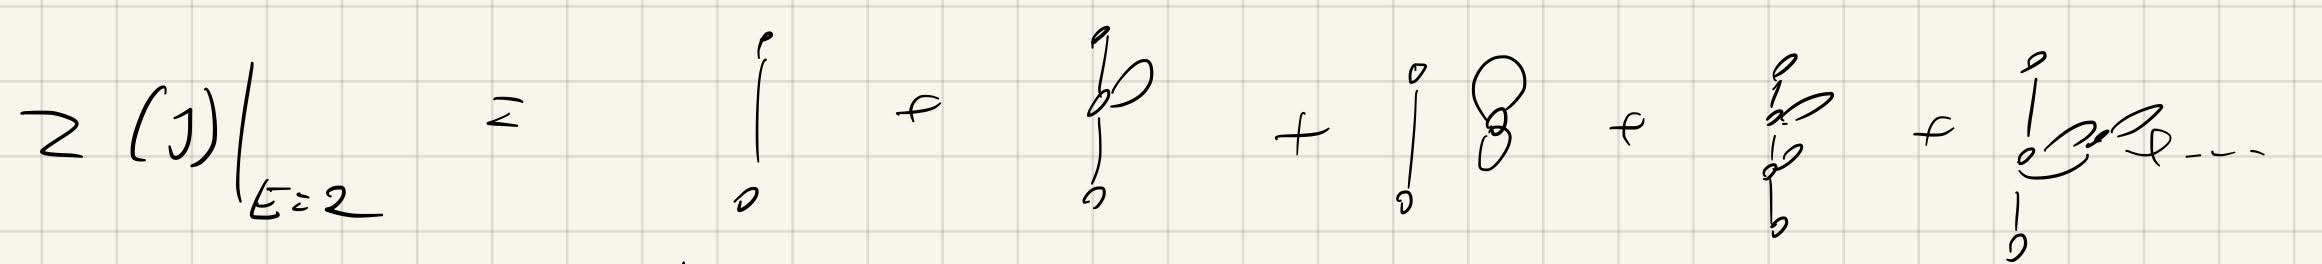
\includegraphics[width=7cm]{res/AQFT/E_2_expansion}
  \label{E_2_expansion}
\end{figure}

where we get disconnected graphs of a different kind, and also get loose outputs
really. Importantly, we can factor out the ``vacuum bubbles'' (or the $E = 0$
case described earlier)

\begin{figure}
  \centering
  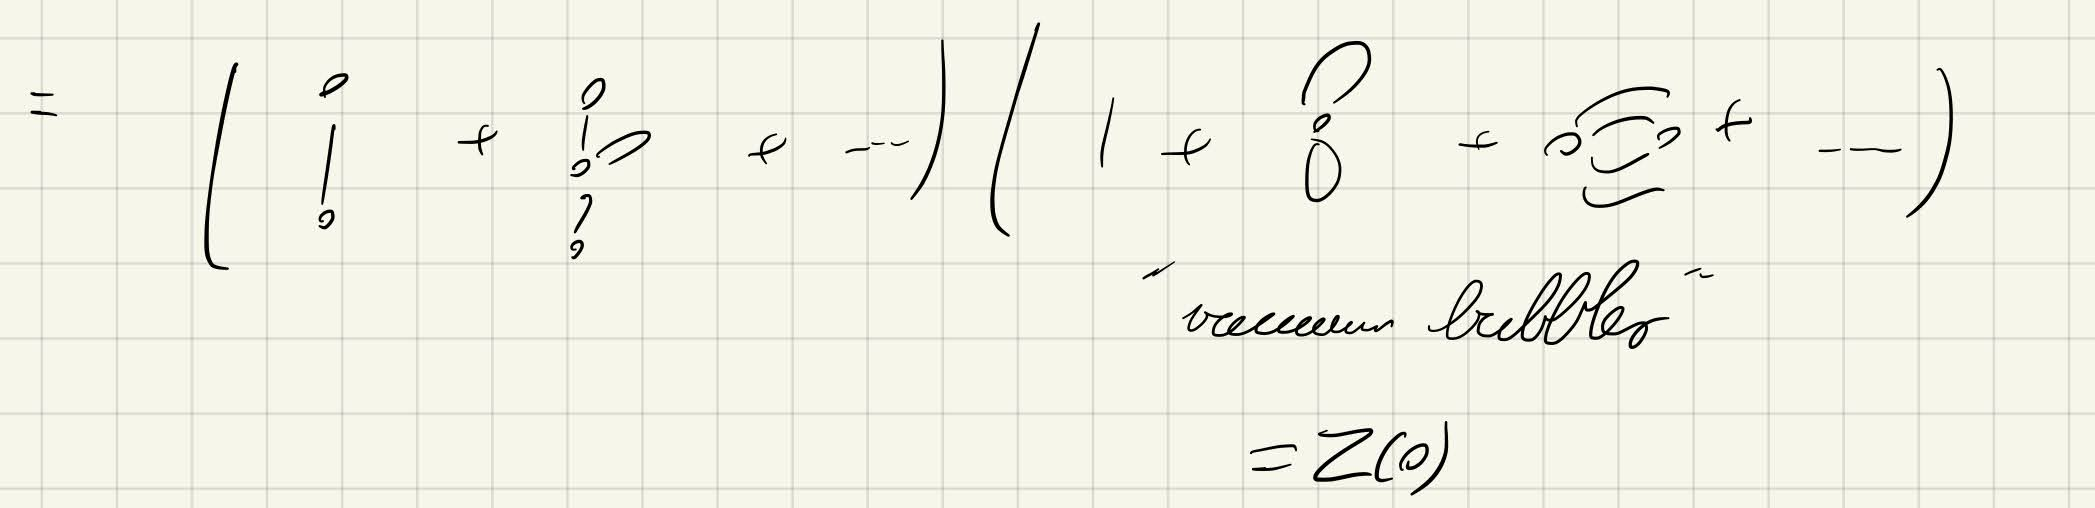
\includegraphics[width=7cm]{res/AQFT/vacuum_bubble_product}
  \label{vacuum_bubble_product}
\end{figure}

Note that this corresponds to the expectation value of $\langle \phi \phi
\rangle$

\begin{figure}
  \centering
  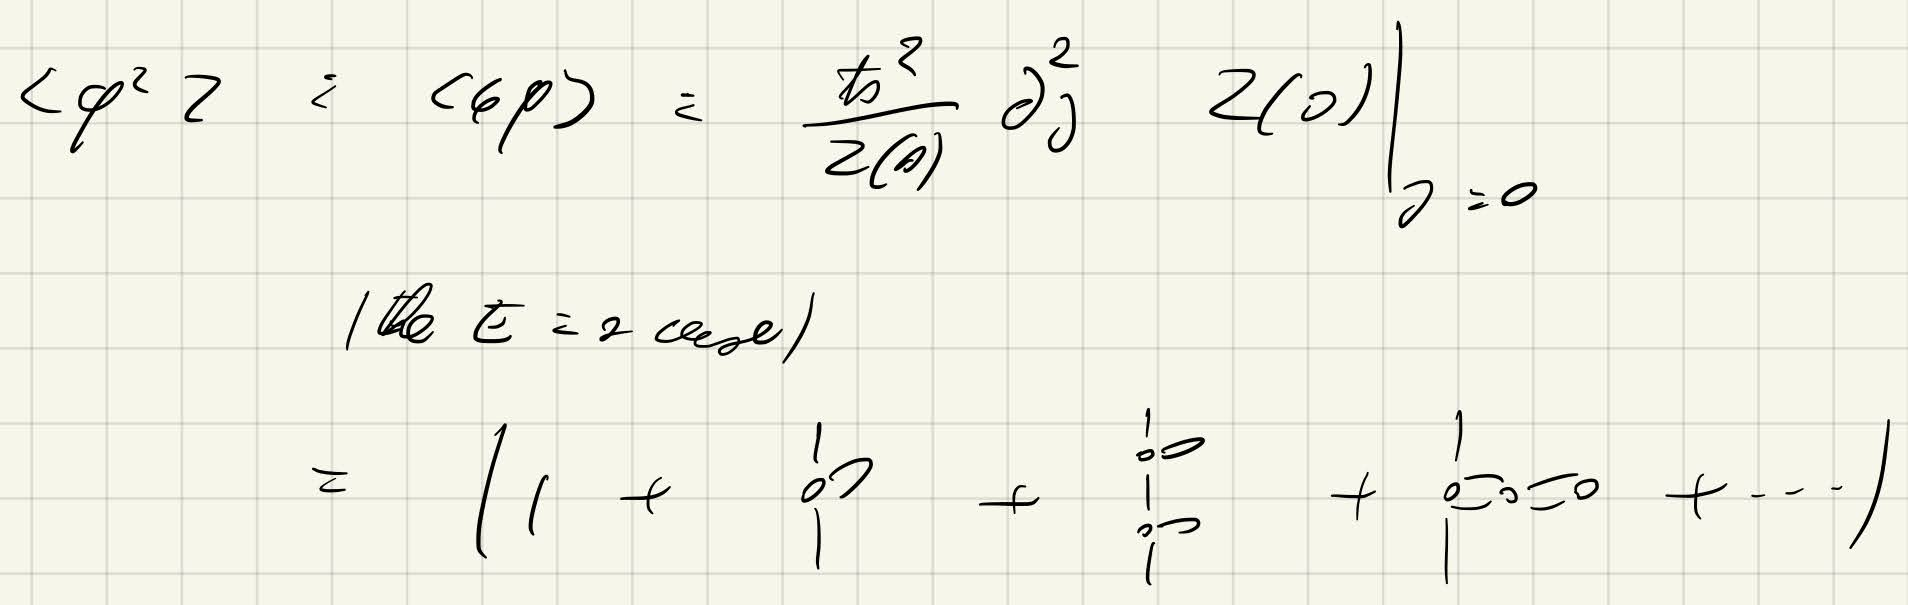
\includegraphics[width=7cm]{res/AQFT/E_2_mean}
  \label{E_2_mean}
\end{figure}

\subsection{Effective Actions}

Our next step is to simplify these calculations by showing that we only have to
work hard on connected graphs. In particular, we define \textbf{effective
  action} $W(J) = -\hbar \ln Z(J)$
and a diagram $D$. Any such $D$ can be written as a product of connect diagrams
as

\begin{equation}
  D = \frac{1}{S_D} \prod_i (C_i)^{n_i}
\end{equation}

where each $C_i$ is a distinct diagram, and we assume each $C_i$ contains its
own symmetry factor, meaning that $S_D = \prod_i n_i!$ is only the number of
ways to rearrange the various connected diagrams. Consequently,

\begin{align*}
  \mathcal{Z} / \mathcal{Z}_0
  &= \sum_{\{n_i\}} \prod_i \frac{1}{n_i!} (C_i)^{n_i} \\
  &= \prod_{i=1}^\infty \sum_{n_i} \frac{1}{n_i!} (C_i)^{n_i} \\
  &= e^{\sum_i C_i} \\
  &= e^{-(W - W_0) / \hbar}
\end{align*}

leaving

\begin{equation}
  \mathcal{Z} / \mathcal{Z}_0 = e^{\sum_i C_i} = e^{-(W - W_0) / \hbar}
\end{equation}

which is quite a remarkable decomposition into only connected graphs. [End of
lecture 4] Let's work out how to use the effective action, $W$ in general.

\begin{example}
  Consider 0-dimension action with two fields
  \begin{equation}
    S(\phi, \chi) = \frac{m^2}{2} \phi^2 + \frac{M^2}{2} \chi^2 +
    \frac{\lambda}{4} \phi^2 \chi^2
  \end{equation}
  which has Feynman rules
  \begin{figure}[H]
    \centering
    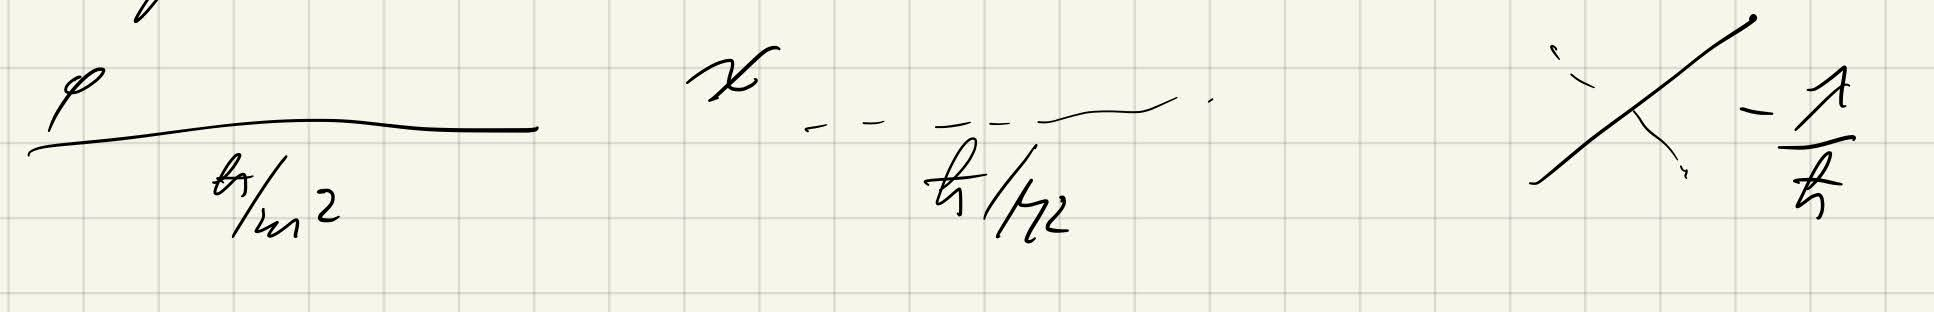
\includegraphics[width=8cm]{res/AQFT/lec_5_effective_action_feynman_rules}
    \caption{Feynman Rules}
    \label{lec_5_effective_action_feynman_rules}
  \end{figure}
  and so we have a sum of connected diagrams given by
  \begin{figure}[H]
    \centering
    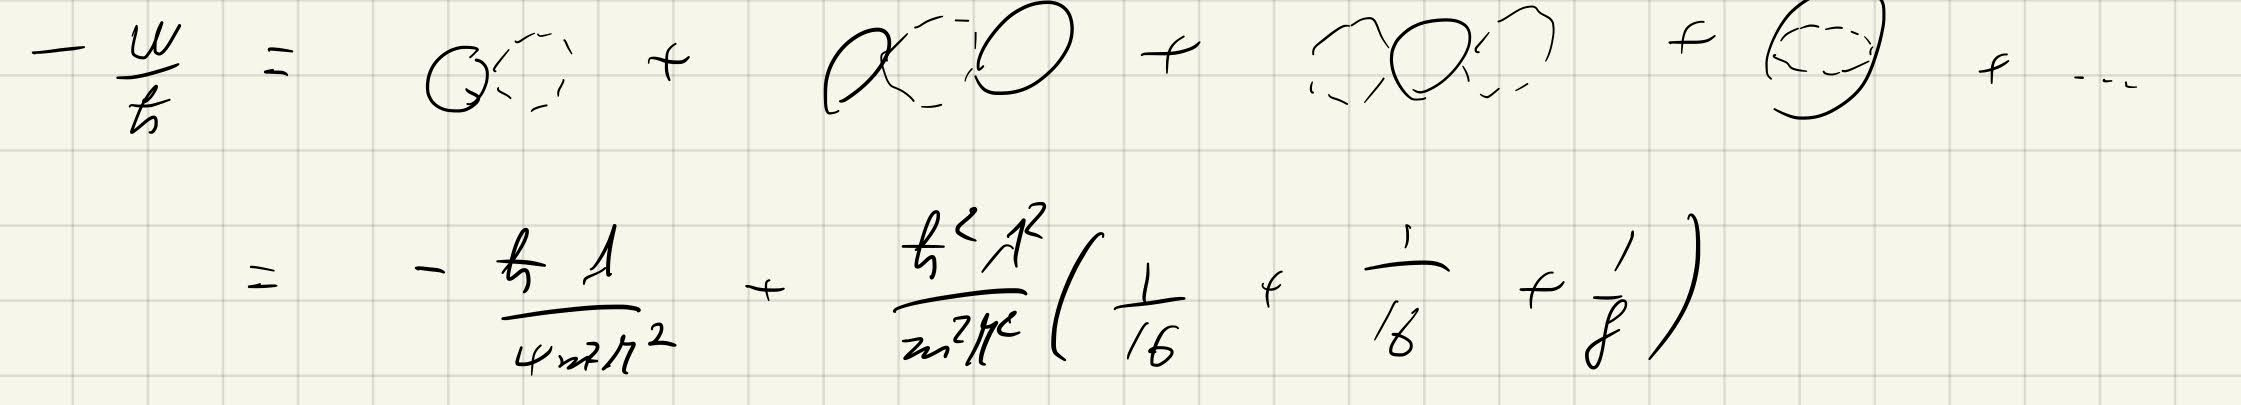
\includegraphics[width=8cm]{res/AQFT/lec_5_connected_diagrams}
    \caption{Connected Diagrams Expansion}
    \label{lec_5_connected_diagrams}
  \end{figure}
  in the so-called ``full theory''. Note here that the free theory involves
  \begin{figure}[H]
    \centering
    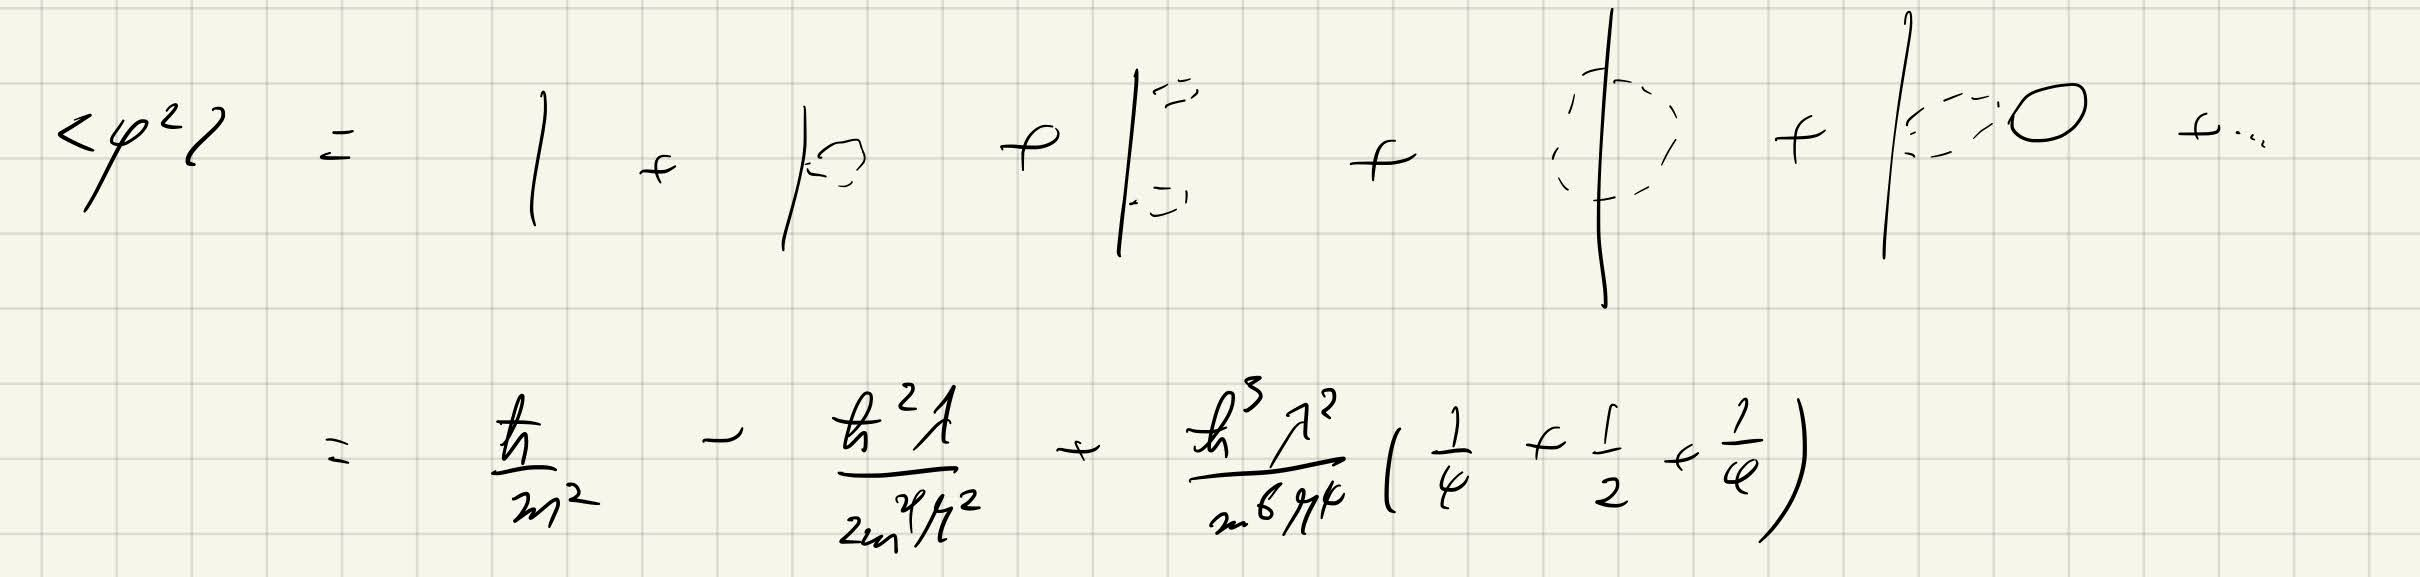
\includegraphics[width=8cm]{res/AQFT/lec_5_free_theory}
    \caption{Free Theory Expected Value}
    \label{lec_5_free_theory}
  \end{figure}

  We can reduce the complexity of these calculations by removing the explicit
  $\chi$ depending by ``integrating it out'' (which can make sense if $\chi$ is
  very massive, for example, so doesn't contribute strongly), then we define our
  effective action to be $W(\phi)$ such that
  \begin{equation}
    e^{-W(\phi) / \hbar} = \int d\chi e^{-S(\phi, \chi) / \hbar}
  \end{equation}
  where we in effect treat $\phi^2 \chi^2$ as a local source for $\chi^2$ (with
  $J = - \phi^2 \lambda / 4$). Consequently, correlatino functions are given by
  \begin{equation}
    \langle f(\phi) \rangle
    = \frac{1}{\mathcal{Z}} \int d \phi d \chi f(\phi) e^{-S(\phi, \chi) / \hbar}
    = \frac{1}{\mathcal{Z}} \int d \phi f(\phi) e^{-W(\phi) / \hbar}
  \end{equation}
  In this special case, we can evaluate the integral explicitly as
  \begin{equation}
    \int d\chi e^{-S(\phi, \chi) / \hbar} = e^{-m^2 \phi^2 / 2 \hbar}
    \sqrt{\frac{2 \pi \hbar}{M^2 + \lambda \phi^2 / 2}}
  \end{equation}
  meaning
  \begin{equation}
    W(\phi) = \frac{1}{2} m \phi^2 + \frac{\hbar}{2}
    \ln(1 + \frac{\lambda}{2M^2} \phi^2) + \frac{\hbar^2}{2}
    \ln \left( \frac{M^2}{2 \pi \hbar} \right)
  \end{equation}
  Here the last constant term does not effect QFT, and is ignored. It does,
  however, have interpretations relating to the energy density of the universe,
  and thus, the cosmological constant. Expanding in $\phi$ (since $\phi = 0$ is
  the local minimum here) gives
  \begin{equation}
    W(\phi) = \frac{m_{eff}^2 \phi^2}{2} + \frac{\lambda_4}{4!} \phi^4 + \dots +
    \frac{\lambda_{2k}{(2k)!}} \phi^{2k}
  \end{equation}
  where $m_{eff}^2 = m^2 + \frac{\hbar \lambda}{4M^2}, \lambda_{2k} = (-1)^{k +
    1} \hbar \frac{(2k)!}{2^{k + 1}k} \frac{\lambda^k}{M^{2k}}$. (notice how we
  get many more terms in the effective theory than the full theory. This is a
  standard effect.). However, integration, as done here, is usually not
  possible, so we resort to pertubations, treating $
  \frac{\lambda}{4} \phi^2 \chi^2$ as a source with rules
  \begin{figure}[H]
    \centering
    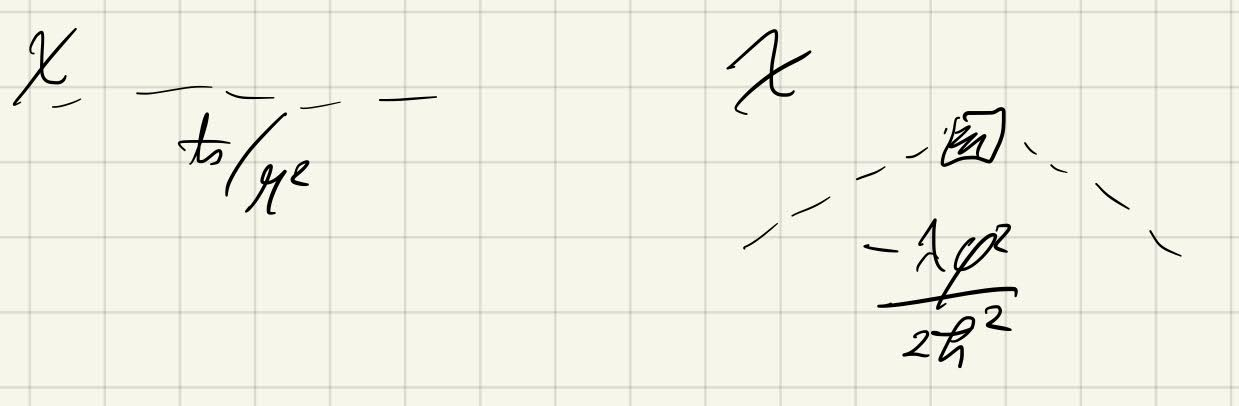
\includegraphics[width=8cm]{res/AQFT/lec_5_effective_source}
    \caption{$\frac{\lambda}{4} \phi^2 \chi^2$ as a source}
    \label{lec_5_effective_source}
  \end{figure}
  leaving
  \begin{figure}[H]
    \centering
    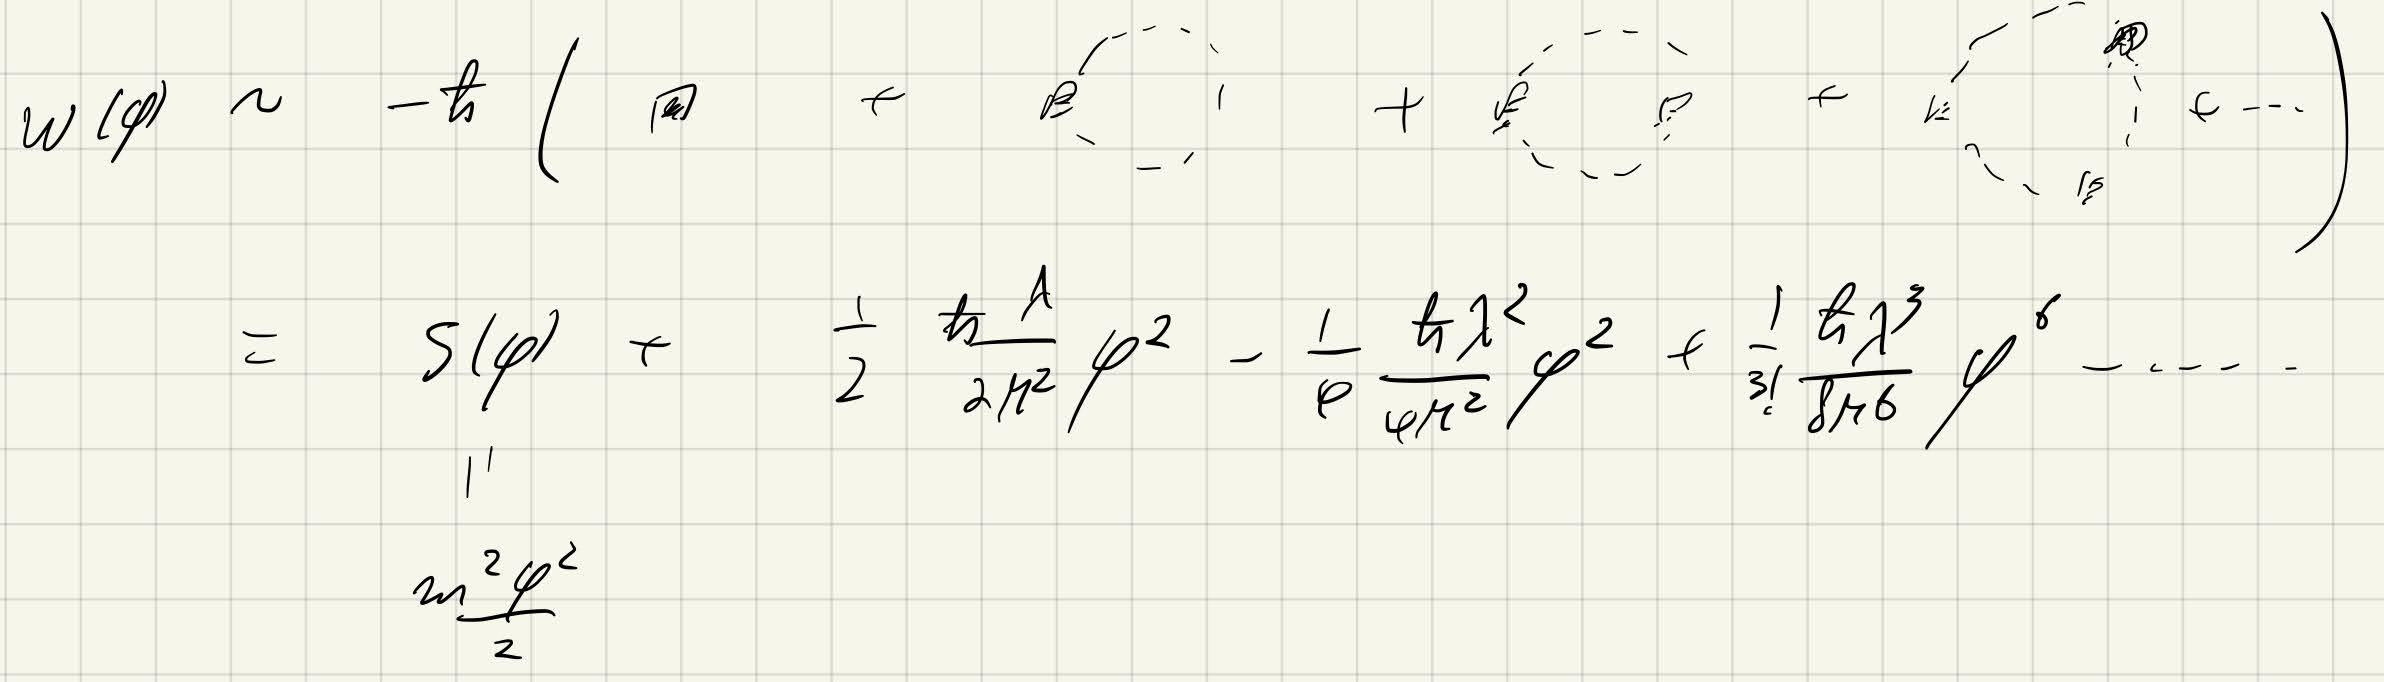
\includegraphics[width=8cm]{res/AQFT/lec_5_effective_pertubation}
    \caption{Effective Action Expansion}
    \label{lec_5_effective_pertubation}
  \end{figure}
  which as usual can be used to calculate correlation functions
  \begin{figure}[H]
    \centering
    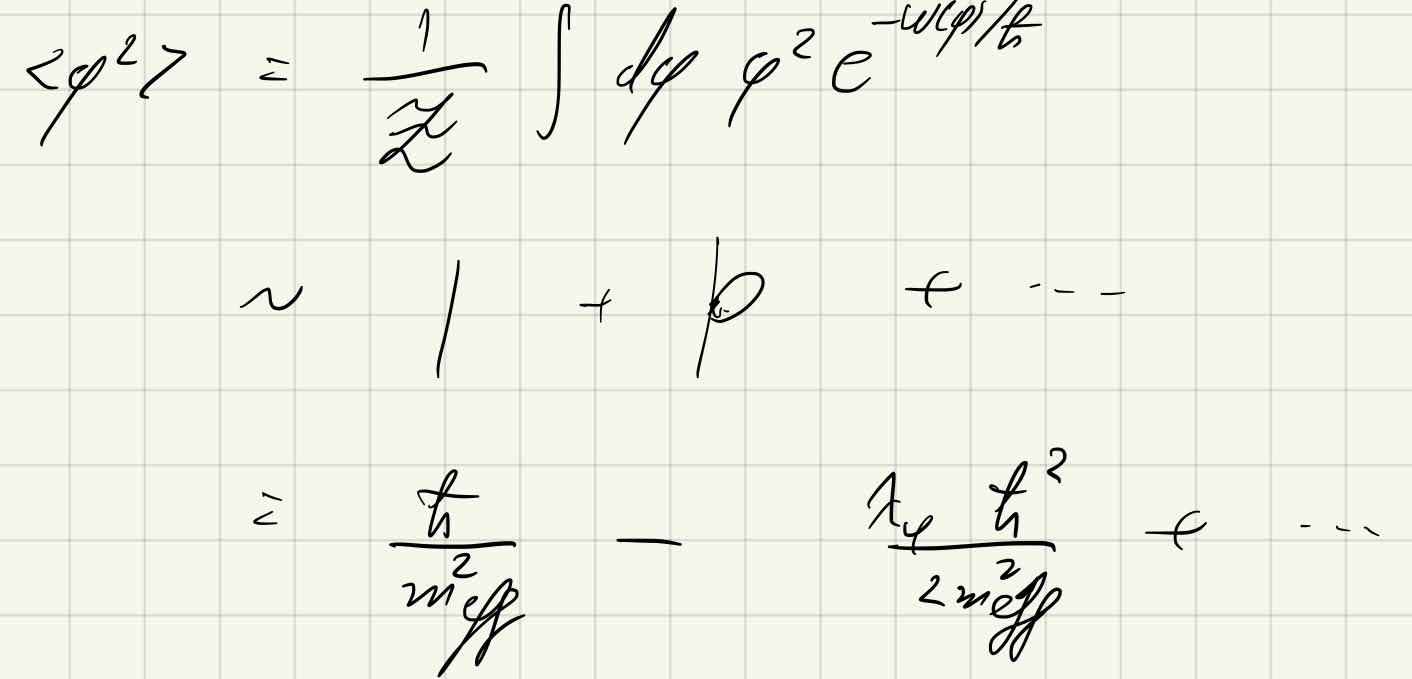
\includegraphics[width=8cm]{res/AQFT/lec_5_effective_correlation}
    \caption{Effective Action Correlation}
    \label{lec_5_effective_correlation}
  \end{figure}
  which is the same as the full theory.
\end{example}

\subsection{Quantum Effective Action $\Gamma$}

The previous effective action accounts for some quantum effects, we can also
introduce the quantum effective action, which accounts for all quantum effects
(?). As such we first define
\begin{equation}
  \Phi = -\partial_J W = \langle \phi \rangle
\end{equation}
for $J \neq 0$. Then we can do a Legendre transform (we assume convexity, and in
practice, this is justified)
\begin{equation}
  \Gamma(\Phi) = W(J) + \Phi J
\end{equation}
which has the property that $\partial_\Phi \Gamma = J$ (so at $J = 0$ we get
$0$, meaning we have a local extremum). In higher dimensions, we can use this to
define the \textbf{effective/quantum} potential $V(\Phi)$ which can be more useful than
the action
\begin{equation}
  \Gamma(\Phi) = \int d^4x \left( -V(\Phi)
    - \frac{1}{2} \partial^\mu \Phi \partial_\mu \Phi + \dots \right)
\end{equation}

We can draw analogies to statistical mechanics with this Legendre transform, and
the Gibbs free energy, for example. [End of lecture 5]

\end{document}